%!TEX root = jsba_main.tex
% Results

\section{Results}
\label{sec:res}

This Section reports and presents the findings of the query execution time measurements. Appendix~\ref{app:queries} lists all queries that were executed
for each implementation without flexible answering and Appendix~\ref{app:flexqueries} lists the queries that were executed flexibly with the previously described
query generalization (cf. Section~\ref{sec:meth_fqa_qgen}). For both developed approaches (cf. Section~\ref{sec:impl_alter}), different horizontal fragmentations
based on the underlying clustering were also investigated. The different fragmentations are caused by restricting the size of the term set 
(cf. Appendix~\ref{app:terms}) to only the first 10 or 30 terms or all 100 terms. Furthermore, the size of the database was scaled for each implementation with
a scaling factor (SF) of 1 up to 10000 that is multiplied with the default number of \verb!INFO! tuples (50) and the default number of \verb!ILL! tuples (100),
i.e. on average each patient has two diseases.

The following bar charts display the average query execution time of a query in milliseconds on the y-axis in dependence on the different scaling factors shown
on the x-axis. In the legend, the different implementations are listed whereas "Materialized" and "Partitions" refer to the first 
(cf. Section~\ref{sec:impl_alter_mater}) and second (cf. Section~\ref{sec:impl_alter_...}) approach, respectively, and the attached numbers indicate the size of 
the underlying term set (10, 30 or 100).
Figure~\ref{fig:query1} shows the average execution time of the first query. As this query is only selecting the average age of all persons in the database, there
can not be performed any intelligent execution based on the similarity metric together with the clustering of the data. Only for the last two scaling factors, 
there is a noticeable increase in the execution time because the amount of data to be scanned also increased. The outlier (Partitions100, SF=10000) might be 
caused by an accidentally imbalanced or adverse distribution of the data across the partitions in contrast to the other implementations.
\begin{figure}[h]
    \centering
    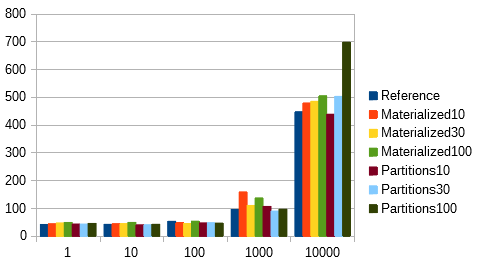
\includegraphics[scale=0.8]{charts/Query1.png}
    \caption{Average query execution time in milliseconds of Query 1 (Appendix~\ref{app:queries}) for SF from 1 up to 10000}
    \label{fig:query1}
\end{figure}

For the second query, the reference implementation's average query execution time took with increasing relation sizes always longer than any implementation 
of the developed approaches (cf. Figure~\ref{fig:query2}). Even for the smaller scaling factors except for the SF of 1, the execution time was slightly longer 
and for the highest scaling factor the execution time of almost five seconds was approximately 50 times as long as the other execution times. This is because the
reference implementation is unlike the developed approaches not capable of answering queries similarity-based as it lacks the clustering-based fragmentation for
the relaxation attribute. The developed approaches, on the contrary, are able to perform similarity-based query answering (cf. Section~\ref{sec:meth_sbqa}) for 
this query as it contains a selection condition on the relaxation attribute. Thus after identification of the relevant fragment and query rewriting, the query 
execution is optimized.

To demonstrate the small differences in the query execution time for the other approaches, the next chart (Figure~\ref{fig:query2withoutref}) plots the same
execution times without the measurements of the reference implementation that are beyond the scope. Two interesting things illustrated in this chart are that,
firstly, both approaches approximately coincide with the execution times and, secondly, both approaches have their fastest execution times (SF=1000 and SF=10000)
for the whole term set compared to the other term set sizes. This is due to the fact that if there are less terms underlying the clustering, then more patient's 
will have a tuple in the \verb!ILL! relation with the disease term \verb!'Liver Failure'! as the data is generated completely randomly and diseases are picked 
randomly from the chosen term set. This results in more tuples matching the selection condition and also more tuples that have to be joined, whereas the 
join is still pretty fast due to collocation, but a presumably bigger result set has to be transferred back to the client.
\begin{figure}[h]
    \centering
    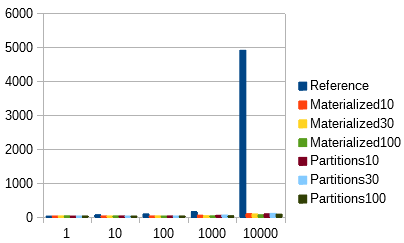
\includegraphics[scale=0.88]{charts/Query2.png}
    \caption{Average query execution time of Query 2 (Appendix~\ref{app:queries})}
    \label{fig:query2}
\end{figure}
\begin{figure}[h]
    \centering
    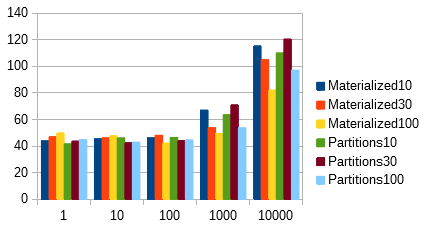
\includegraphics[scale=0.88]{charts/Query2WithoutReference.png}
    \caption{Average query execution time of Query 2 (Appendix~\ref{app:queries}) without reference implementation}
    \label{fig:query2withoutref}
\end{figure}


ASdf
\begin{figure}[h]
    \centering
    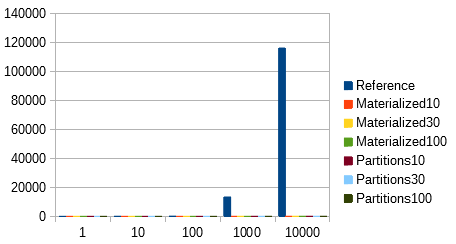
\includegraphics[scale=0.9]{charts/Query3.png}
    \caption{Average query execution time of Query 3 (Appendix~\ref{app:queries})}
    \label{fig:query3}
\end{figure}

\begin{figure}[h]
    \centering
    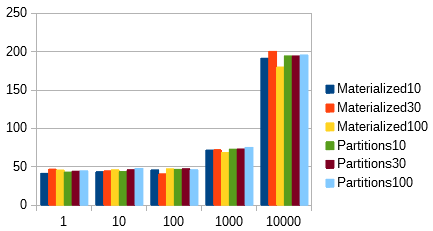
\includegraphics[scale=0.9]{charts/Query3WithoutReference.png}
    \caption{Average query execution time of Query 3 (Appendix~\ref{app:queries}) without reference implementation}
    \label{fig:query3withoutref}
\end{figure}